\documentclass{article}

\usepackage{amsmath}
\usepackage{amssymb}
\usepackage{amsfonts}
\usepackage{mathtools}
\usepackage{graphicx}

\title{Engine Dynamics}
\author{Camilo Garc\'ia}

\begin{document}
\maketitle
\section{Problem Description and Data}\label{sec:Problem Description and Data} % (fold)
A long time ago, in a galaxy far far away. That is, during my masters degree circa 2013, we did a dynamometer test of a front wheel drive vehicle to get the torque-speed-power curves of the internal combustion engine. This was the final project of a vehicle dynamics course, and fortunately, I was able to dig out the data from the experiment to show my abilities as dynamical systems and control engineer. For this example, I can only show my abilities to model dynamical systems. So, lets begin with a description of the experiment.
\subsection{The Vehicle and the Environment}\label{sub:The Vehicle} % (fold)
The test subject was a 2007 Ford Fusion. A front wheel drive vehicle equipped with a four stroke V6 engine that displaces a volume of 3 liters. According to the technical specification, the engine of this vehicle should be capable of producing a maximum 221 metric horse-power, i.e., 162.5 [kW] at 6250 [RPM], and a maximum torque of 278 [Nm] at  at 4800 [RPM], sea level, when new. All these power gets to the front wheels via a torque converter automatic gearbox.

After 5 years of use, in an altitude of 2600 [m] above sea level (yes, Bogot\'a is a city up in the clouds), and a power delivery via the automatic gearbox, the measured torque and calculated power will definitely be way lower. Lets see.
% subsection The Vehicle (end)
\subsection{The data}\label{sub:The data} % (fold)
The testing rig is a four wheel drive 2000 [hp] axle-hub dynamometer, with Dyno-max Pro software acquisition software. This combo can provide temperature, atmospheric pressure and relative humidity measurements to make the test compliant with the SAR J1349 Engine Test Power Code. In an ideal world, we could have taken all those factors into consideration. For this test though, those variables were not available.

The axle-hub dynamometer has an Eddy current absorber able to provide a steady state RPM value according to the provided current, varying the absorber load, this is the input to the system. For the outputs, we have the torque measurement at the axle, and the RPM of the engine.

Again, in an ideal world where we would have a measurement of the output torque throughout the whole range of engine RPM. Unfortunately, this is not the case. When testing, we did not have a proper gas extraction system, the test rig had a single hose for gas extraction, while the vehicle had double exhaust pipes (no worries, the garage at the laboratory had a good ventilation system). Then, for security reasons we had a single run of test. In addition, it was not possible to make an automated test setting up a ladder of RPM values throughout the whole range because we did not have the knowledge to set it up. Then, we opted for a manual variation of the coil current to measure the torque and RPM output at 9 different absorber RPM values for within 2000 and 4000 RPM of the engine. Definitely not an ideal situation because we are not even at the RPM value for max torque. Making this exercise much more interesting.

Let see a picture of the experimental data to get a clearer \textit{picture} of the problem at hand. Figure~\ref{fig:data} shows the motor RPM, and the torque measurement at the absorber according to the different RPM of the absorber.
\begin{figure}[ht]
	\centering
	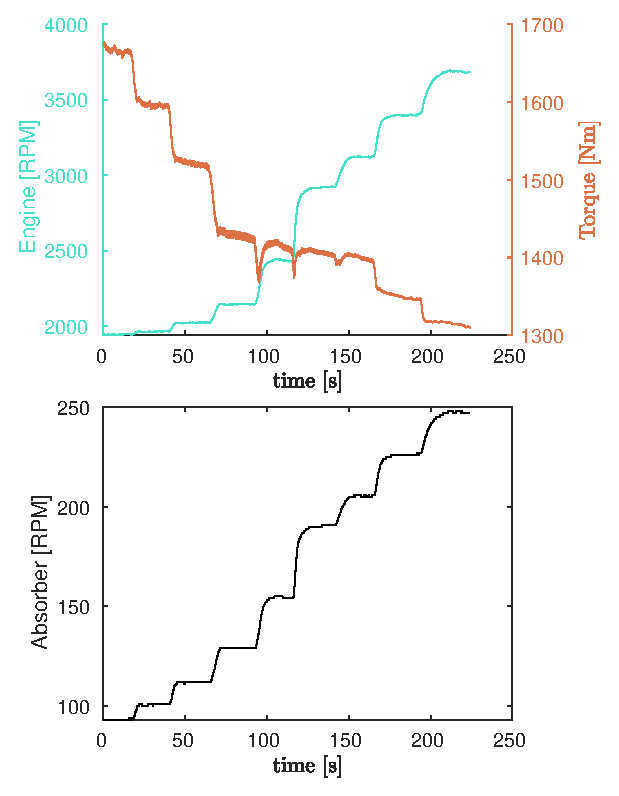
\includegraphics[width=0.7\linewidth]{./figures/data_fig.eps}
	\caption{Outputs: Motor RPM and Torque. Input: Absorber RPM}
	\label{fig:data}
\end{figure}

So, one experiment for a not so ideal range of RPM, from a non so systematic test, with some questionable behavior around 2500 RPM of the engine. 

Other consideration include: The gear in which the vehicle was during the test is unknown. With the power google, I have the ratios for each gear, the final drive ratio, and the information that these tests are normally in third gear.

\begin{table}
	\caption{Gear ratios}\label{tab:gear_ratios}
	\begin{center}
		\begin{tabular}[c]{l|l|l}
			\hline
			Gear Ratios & five-speed & six-speed \\
			\hline
			1st & 3.31 & 4.10 \\
			3rd & 1.23:1 & 1.56:1 \\
			Final Drive & 4.39:1 & 3.46:1 \\
			\hline
			1st$\times$Final & 14.53 & 14.35 \\
			3rd$\times$Final & 5.39 & 5.39 \\
			\hline
		\end{tabular}
	\end{center}
\end{table}

Let us see what we can make out of this data.
% subsection The data (end)
\subsection{Objectives}\label{sub:Objectives} % (fold)
\paragraph{Test my algorithm:}\label{par:Test my algorithm} % (fold)
I have a \textbf{data-driven} development, notice the emphasis on data-driven, this is not within the traditional \textit{machine learning} (ML) methods or what the mainstream media is calling AI. It is called (drum-roll please); the \textit{extended dynamic mode decomposition} (EDMD) with pq-quasi norm reduction or, as I like to call it: the pqEDMD.  
% paragraph Test my algorithm (end)
\paragraph{Apply traditional identification methods:}\label{par:Apply traditional identification methods} % (fold)
On top of EDMD based identification methods, I have extensive knowledge of traditional modeling and identification techniques. Then, what can we do with the information from the data, and the model from the pqEDMD.
% paragraph Apply traditional identification methods (end)
% subsection Objectives (end)
% section Problem Description and Data (end)
\section{The pqEDMD}\label{sec:The pqEDMD} % (fold)
Without getting too technical, the pqEDMD is an algorithm that takes \textit{input/output} data from an arbitrary system and produces an approximation of its dynamics using a family of polynomial functions, and a mathematical structure similar to a linear system identification, that is, we get an A, B, C and maybe D matrices. Although is similar to a linear identification, this method captures the nonlinear behavior of a dynamical system. Where the A matrix is called an operator, because it acts on a set of functions (the polynomial functions) and not directly on the states, like in a linear system.

Figure~\ref{fig:pqEDMD_appx} shows the result of applying the pqEDMD algorithm to the data-set. The testing methodology is equivalent to an initial value problem in dynamical systems. From the same initial condition, the algorithm applies the same sequence of inputs that drive the experimental data. Therefore, there will be some error, not this much error, but still, some deviation from the actual curves. To be clear about this point, this is not a one step look ahead predictor, the evolution is just from the same initial condition.

\begin{figure}[ht]
\centering
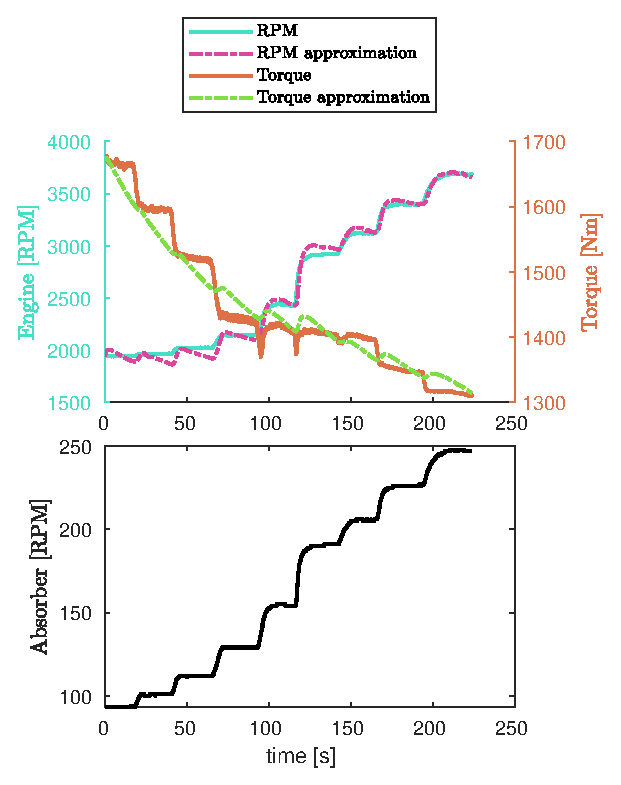
\includegraphics[width=0.7\linewidth]{./figures/appx_fig.eps}
\caption{pqEDMD approximation of the Engine Dynamics}
\label{fig:pqEDMD_appx}
\end{figure}

Not being able to have a better approximation came as a surprise for me. The algorithm is generally much better at identifying dynamical systems from data. What is happening then? 

It would be necessary to go deeper into the analysis and possible refinement of the parameters to make the approximation. What is definitely true, is the fact that the whole system has many interconnected parts. The engine has its dynamics, then we have the torque converter and planetary gearbox dynamics before we get the shaft. The torque measurement at the shaft, also depends on the dynamics of the dynamometer; there is a feedback control loop that maintains a constant RPM at the absorber for a set value of the break current. This is not a strictly open loop system. 

On top not having an open loop system, we also have to consider the gearbox dynamics. In a perfect world, we would have just an efficiency factor from the effect of the gearbox. Lets see then the behavior of the absorber RPM vs., the engine RPM. 
\subsection{Gearbox analysis}\label{sub:Gearbox analysis} % (fold)
This exercise is about the estimating the engine torque and eventually calculating the power at different RPM. For this, we could say that the engine RPM is is proportional to the absorber RPM. Lets check this hypothesis. Figure~\ref{fig:RPMs} shows the plots of the absorber RPM vs., engine RPM and the ratio between the two. It is clear, that at low RPM, the ratio is not linear, and therefore it is not just proportional. At high RPM we can confirm that that test was in first gear. So, we have to consider the gearbox dynamics on to of the engine dynamics to do an analysis. 

\begin{figure}[ht]
\centering
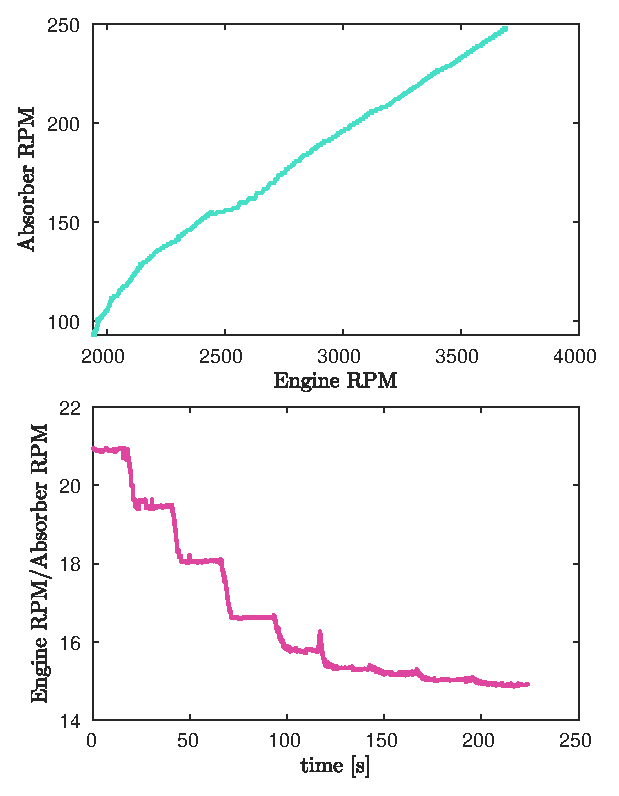
\includegraphics[width=0.7\linewidth]{./figures/ratio_fig.eps}
\caption{Engine RPM vs., Absorber RPM, and ratio between the two.}
\label{fig:RPMs}
\end{figure}

Knowing that is necessary to consider all of these dynamics to perform the analysis, my hypothesis is that there are some unobservable dynamics from the output, making an analysis like the pqEDMD not relevant to this problem.

The data driven analysis is not all we have. We still have traditional identification methods.
% subsection Gearbox analysis (end)
\subsection{Higher order models}\label{sub:Higher order models} % (fold)
The pqEDMD allows for higher order models. The model in Section~\ref{sec:The pqEDMD} shows the best approximation that fits the data. After evaluating the performance of other decompositions coming from different parameterizations, we get approximations where the shape suggests that a better data-set could produce more accurate approximations. Consider for example Figure~\ref{fig:another_EDMD_appx}, where the overall error is higher than the approximation in Figure~\ref{fig:pqEDMD_appx} but the overall shape suggest that the algorithm has the potential to produce accurate approximations of this \textit{intput/output} behavior.

\begin{figure}[ht]
\centering
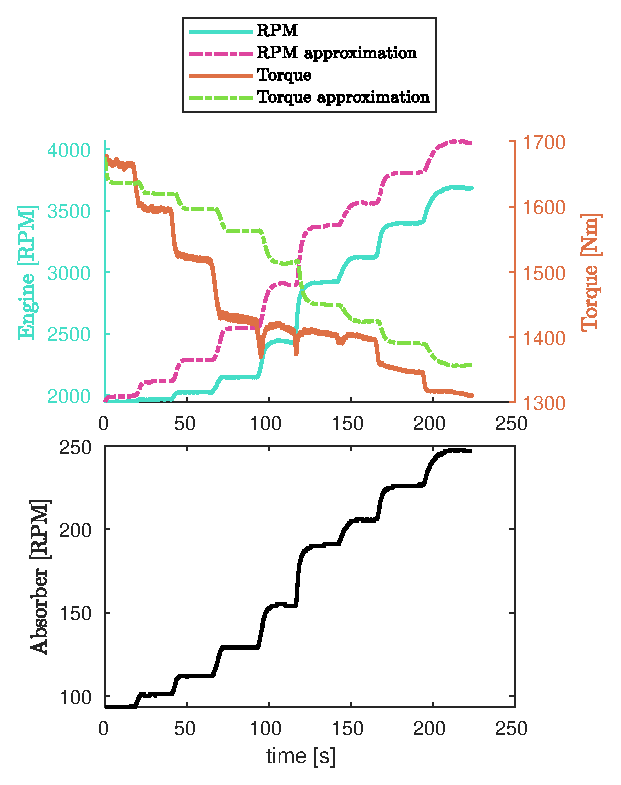
\includegraphics[width=0.7\linewidth]{./figures/appx_alt_fig.eps}
\caption{Alternative approximation of the Drivetrain Dynamics using other parameterizations of the pqEDMD.}
\label{fig:another_EDMD_appx}
\end{figure}

% subsection Higher order models (end)
% section The pqEDMD (end)
\section{Traditional Identification}\label{sec:Traditional Identification} % (fold)
At the time, for the development of the project, the exercise was to get the torque-power vs., RPM curve of the engine. To do this, we take the values of the torque at ``steady state'' for each step, take an average and divide by the gear ratio to get the torque at the engine for the different RPM values. For the power, just multiply by the engine speed in [rad/s] and plot the result. This is a static analysis and pretty simple and boring. Therefore, I will try to produce a dynamical system of the assembly. 

Defining:
\begin{itemize}
	\item $k_e$: Moment of inertia (and damping effect) of the engine and transmission [kg$\cdot$m$^2$]
	\item $k_d$: Moment of inertia (and damping effect) of the dynamometer and transmission [kg$\cdot$m$^2$]
	\item $\omega_e$: Engine angular velociy [rad$\cdot$s]
	\item $\omega_d$: Absorber angular velocity [rad$\cdot$s]
	\item $T_d$: Torque measured at the absorber [Nm]
\end{itemize}
\subsection{Linear Approximation}\label{sub:Linear Approximation} % (fold)
After some attempts at using an adaptation of~\cite{Blumenschein2013}, and trying to include some transmission model, to account for the torque converter/planerary-gearbox assembly. The results where not satisfactory. Instead, consider a more pragmatic approach:
\begin{itemize}
	\item The engine speed is directly proportional to the absorber speed. 
		\[
			\omega_e \approx k_1\omega_d
		\]
		The constant $k_1$ is related to the gearbox ratio. 
	\item The absorber torque is inversely proportional to the absorber speed.
		\[
			T_d \approx \frac{k_2}{\omega_d}
		\]
		This comes from the analysis of the power equation $P_d=T_d\omega_d$, at steady state, the conservation of power applies, then, if the angular velocity increases, then the torque must decrease.
\end{itemize}
Then, we can approximate the dynamics of the system as:
\begin{align}
	k_e\dot{\omega}_{e} & = k_1\omega_d - \omega_e\\
	k_d\dot{T}_d & = \frac{k_2}{\omega_d} - T_d.
\end{align}

Then, there are four parameters to estimate. The two ``inertias'' and the two proportionality constants. Figure~\ref{fig:linear_appx} shows the validation of the differential equation after identifying the parameters. Even though this is not an accurate model, the overall shape of the response suggests that it is a good starting point to eventually get an approximation of the engine torque.

\begin{figure}
\centering
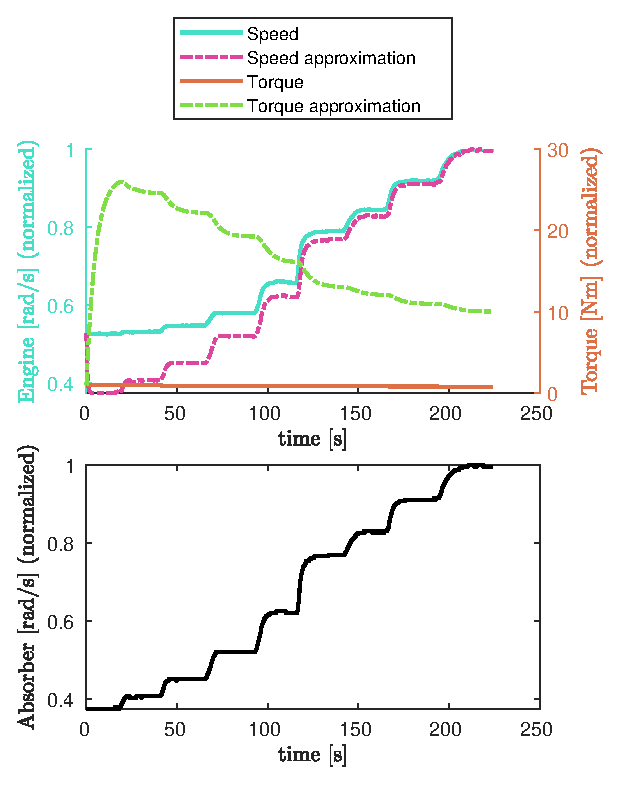
\includegraphics[width=0.7\linewidth]{./figures/trad_appx_fig.eps}
\caption{Linear approximation of the engine speed and absorber torque}
\label{fig:linear_appx}
\end{figure}

% subsection Linear Approximation (end)
% section Traditional Identification (end)
\bibliography{ice_model}
\bibliographystyle{ieeetr}
\end{document}
